\section{Fourier-Theorie}
\todo{Woche 3 - 4.10.21}
\subsection{Fourier-Reihe}
\[
c_n = \frac{1}{T}\int_{T}^{}x(t)*e^{-jn2\pi f_0 t}dt
\]

\subsection{Fourier-Transformation}
\begin{align*}
	X(\omega) &= \mathcal{F}\{x(t)\} = \int_{-\infty}^{\infty}x(t)\cdot e^{-j\omega t}dt \\
	x(t) &= \mathcal{F^{-1}}\{X(\omega)\} = \frac{1}{2\pi}\int_{-\infty}^{\infty}X(\omega)\cdot e^{j\omega t}d\omega \\
\end{align*}

\subsubsection{Eigenschaften}
\begin{enumerate}[nosep]
	\item Linearität $a_1x_1(t) + a_2x_2(t) \transform a_1X_1(\omega) + a_2X_2(\omega)$ 
	\item Verschiebung in Zeit. $x(t - t_0) \transform X(\omega) \cdot e^{-j\omega t_0}$
	\item Verschiebung in Freq. $x(t) \cdot e^{j\omega_0 t} \transform X(\omega - \omega_0)$
	\item Modulationssatz $x(t) \cdot \cos(\omega_0t) \transform \frac{1}{2}X(\omega - \omega_0) + \frac{1}{2}X(\omega + \omega_0)$ \\ $x(t) \cdot \sin(\omega_0t) \transform \frac{1}{2j}X(\omega - \omega_0) + \frac{1}{2j}X(\omega + \omega_0)$ 
	\item Skalierung im Zeit und Freq. $x(k\cdot t) \transform \frac{1}{|k|}X(\frac{\omega}{k})$
	\item Zeit oder Freq Umkehrung $x(-t) \transform X(-\omega)$
	\item Dualität $X(t) \transform 2\pi \cdot x(-\omega)$
	\item Differentiation $\frac{d}{dt}x(t) \transform j\omega \cdot X(\omega)$
	\item Integration $\int_{-\infty}^{t}(x(\tau)d\tau \transform X(\omega)(\frac{1}{j\omega} + \pi \delta(\omega)))$ \\ $\delta(\omega)$: Dirac'sche Impuls
	\item Multiplikation $x_1(t) \cdot x_2(t) \transform \frac{1}{2\pi}\int_{-\infty}^{\infty}X_1(\Omega) \cdot X_2(\omega - \Omega)d\Omega$ \\
	$x_1(t) \cdot x_2(t) \transform \frac{1}{2\pi}X_1(\omega) * X_2(\omega)$
	\item Faltungssatz $\int_{-\infty}^{\infty}x_1(\tau) \cdot x_2(t - \tau)d\tau \transform X_1(\omega) \cdot X_2(\omega)$ \\
	$x_1(t) * x_2(t) \transform X_1(\omega) \cdot X_2(\omega)$
	\item Impulsfunktion $1 \transform 2\pi\delta(\omega)$
	\item $\cos(\omega_0 t) \transform \pi (\delta(\omega - \omega_0) + \delta(\omega + \omega_0))$ \\
	$\sin(\omega_0 t) \transform -j\pi (\delta(\omega - \omega_0) + \delta(\omega + \omega_0))$ \\
	$\sum_{n=-\infty}^{\infty}c_n\cdot e^{jn\omega_0 t} \transform 2\pi \sum_{n=-\infty}^{\infty}c_n \delta (\omega - n \omega_0)$
\end{enumerate}


\subsection{Frequenzbereich: Modulationssatz}
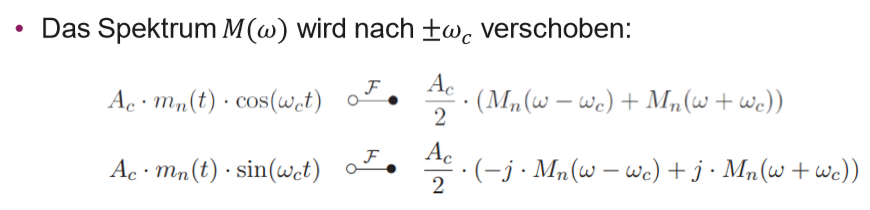
\includegraphics[width=\columnwidth]{Images/screenshot006}

\subsection{Basisbanddarstellung}
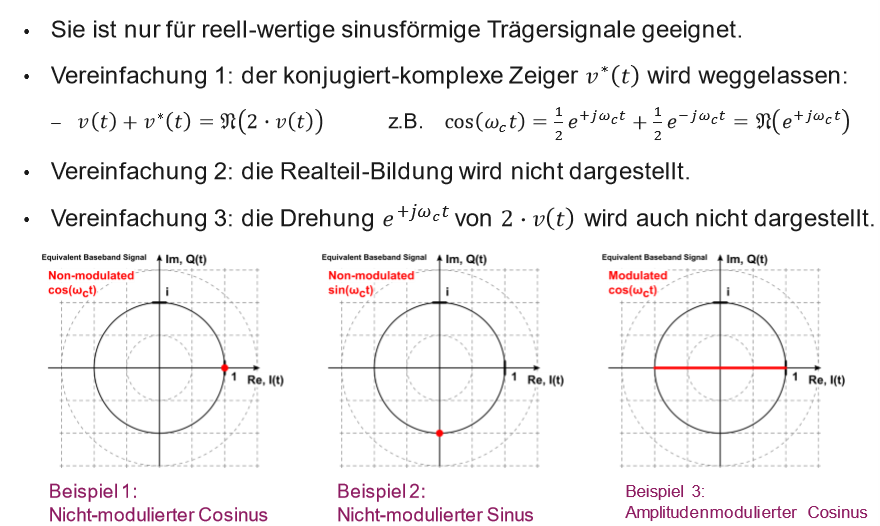
\includegraphics[width=\columnwidth]{Images/screenshot007}
